\documentclass{article}
\usepackage[utf8]{inputenc}
\usepackage{graphicx}
\usepackage{sectsty}

\title{Final Sheet}
\author{}
\date{December 2021}
\renewcommand\thesubsection{\thesection.\alph{subsection}}
\subsectionfont{\fontsize{11}{15}\normalfont}
\renewcommand{\theenumi}{\roman{enumi}}
\usepackage[margin=1in]{geometry}
\begin{document}

\maketitle

\section{Data}

\section{Normal distribution}

\section{Binomial distribution}

\section{Regression Analysis}

\section{Experiments and Observational studies}

\section{Types of sampling}
\section{Hypothesis Testing}
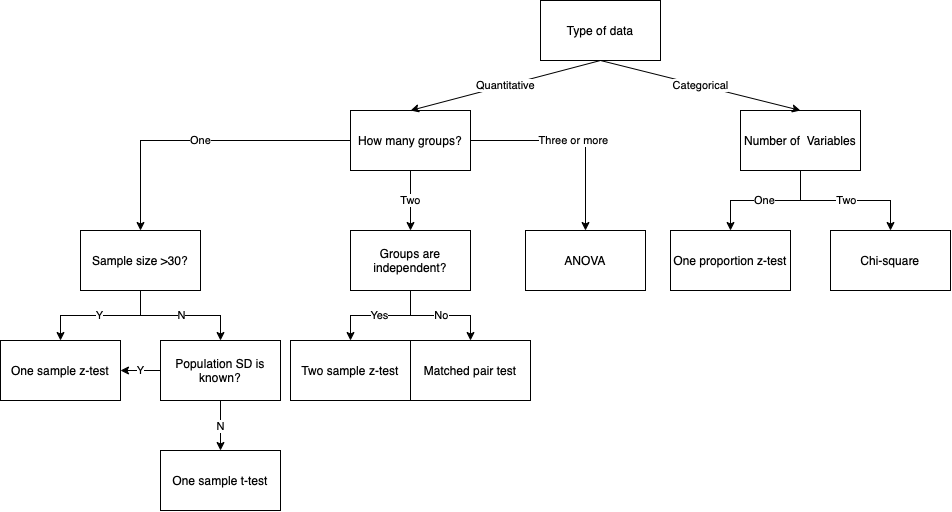
\includegraphics[scale = 0.5]{dec-tree.png}
\subsection{One sample z-test}
\textbf{Algorithm}
\begin{itemize}
\item Idenitify parameter of interest. Find the null and alternative hypotheseses.\\
      s - The standard deviation of the sample.\\
      n - The sample size.\\
      $\mu$ - Hypothethised population mean.\\
      $\mathbf{SE}(\bar{y}) = \frac{s}{\sqrt{n}}$ - Standard error of the statistic.
\item Construct the null-model: $\mathbf{N}(\mu,\frac{s}{\sqrt{n}})$
\item Find the test-statistic(t): $\mathbf{Z} = \frac{x-\mu}{\mathbf{SE}(\bar{y})}$
\item Using R compute the p-value:
\begin{itemize}
    \item One-sided hypothesis : pnorm(t)
    \item Two-sided hypothesis : 2 $\cdot$ pnorm(t)
\end{itemize}
\item If the p-value is less than $\alpha$ - reject the null-hypothesis. 
    Otherwise, you fail to reject the null-hypothesis.
\end{itemize}
\subsection{One proportion z-test}
\textbf{Algorithm}
\begin{itemize}
\item Idenitify parameter of interest. Find the null and alternative hypotheseses.\\
      n - The sample size.\\
      $p_0$ - Hypothethised proportion.\\
      $\mathbf{SD} = \sqrt{\frac{p_0(1-p_0)}{n}}$ - Standard error of the statistic.
\item Construct the null-model: $\mathbf{N}(\mu,\sqrt{\frac{p_0(1-p_0)}{n}})$
\item Find the test-statistic(t): $\mathbf{Z} = \frac{x-p_0}{\mathbf{SD}}$
\item Using R compute the p-value:
\begin{itemize}
    \item One-sided hypothesis : pnorm(t)
    \item Two-sided hypothesis : 2 $\cdot$ pnorm(t)
\end{itemize}
\item If the p-value is less than $\alpha$ - reject the null-hypothesis. 
    Otherwise, you fail to reject the null-hypothesis.
\end{itemize}
\subsection{Two sample z-test}
\textbf{Algorithm}
\begin{itemize}
\item Idenitify parameter of interest. Find the null and alternative hypotheseses.\\
      s - The standard deviation of the sample.\\
      n - The sample size.\\
      $\mu$ - Hypothethised population mean.\\
      $\mathbf{SE}(\bar{y}) = \frac{s}{\sqrt{n}}$ - Standard error of the statistic.
\item Construct the null-model: $\mathbf{N}(\mu,\frac{s}{\sqrt{n}})$
\item Find the test-statistic(t): $\mathbf{Z} = \frac{x-p_0}{\mathbf{SE}(\bar{y})}$
\item Using R compute the p-value:
\begin{itemize}
    \item One-sided hypothesis : pnorm(t)
    \item Two-sided hypothesis : 2 $\cdot$ pnorm(t)
\end{itemize}
\item If the p-value is less than $\alpha$ - reject the null-hypothesis. 
    Otherwise, you fail to reject the null-hypothesis.
\end{itemize}
\subsection{Matched pair}
\subsection{One sample t-test}
\subsection{ANOVA}


\end{document}